%!TEX root = ../Thesis.tex


\section{Use-Cases  \textcolor{blue}{[Julius Figge]}}

Im Nachfolgenden sind die Use-Cases des Programms dargestellt (siehe \cref{fig:usecases}).
Diese sind den Projektvorgaben entnommen.\footnote{Vgl. \cite{Vorgaben2020}}

\begin{figure}[hbt]
    \label{usecase}
    \centering
    \begin{minipage}[t]{1\textwidth}
        \caption{Use-Case Diagramm}
        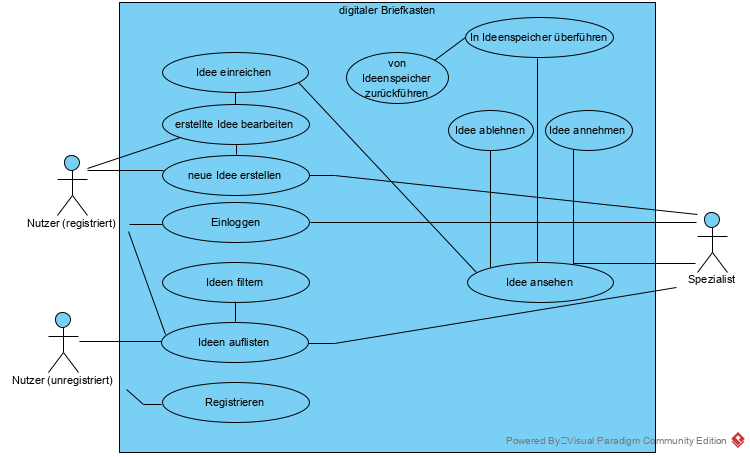
\includegraphics[width=1\textwidth]{img/createAnAccountWithSpamMailAccountYouSucker.png}\\
        \source{Eigene Darstellung}
        \label{fig:usecases}
    \end{minipage}
\end{figure}

Für das Use-Case Diagramm sind drei Rollen von Relevanz.
Zuerst der \texttt{unregistrierte Nutzer}, was den Zugriff ohne besondere Rechte darstellt.
Des weiteren der \texttt{eingeloggte Nutzer} der mehr Möglichkeiten hat. Hierzu gehört auch der \texttt{Administrator}.
Dieser hat über die Möglichkeiten des Nutzers hinaus weitere administrative Rechte.\footnote{Der Admin ist als eigener Use-Case im Anhang dargestellt. Siehe Anhang \ref{Anhang-Admin} auf S.\pageref{Anhang-Admin}}
Jedoch besitzt er nicht die Rechte der dritten Rolle des \texttt{Spezialisten}.\\

Die Use-Cases lassen sich in zwei \enquote{Kern}-Kategorien unterteilen.
Das sind zunächst die \texttt{Account} bezogenen Use-Cases.\\
Hierzu gehören der Vorgang des Einloggens sowie das Registrieren. Zu diesem ist anzumerken, dass Spezialisten sich lediglich einloggen können.
Durch ihre weitreichenden Rechte dürfen diese sich nicht normal registrieren, sondern werden durch den Administrator angelegt.\\
Der zweite Use-Case ist die \texttt{Erstellung und Verwaltung von Ideen}.\\
Eingereichte Ideen lassen sich durch alle Nutzer jeder Rolle einsehen und filtern. Darüber hinaus haben alle eingeloggten Nutzer die Möglichkeit Ideen zu erstellen, zu bearbeiten und zur Bewertung einzureichen.\\
Diese eingereichten Ideen werden durch Spezialisten bewertet oder gespeichert.

Des weiteren existiert die Möglichkeit, für alle Nutzer, dem Administrator der Plattform über ein Kontaktformular Nachrichten zu senden.\footnote{Das zugehörige Use-Case Diagramm findet sich im Anhang \ref{Anhang-Kontakt} auf S.\pageref{Anhang-Kontakt}}